% !TEX TS-program = pdflatex
% !TEX encoding = UTF-8 Unicode

% This file is a template using the "beamer" package to create slides for a talk or presentation
% - Talk at a conference/colloquium.
% - Talk length is about 20min.
% - Style is ornate.

% MODIFIED by Jonathan Kew, 2008-07-06
% The header comments and encoding in this file were modified for inclusion with TeXworks.
% The content is otherwise unchanged from the original distributed with the beamer package.

\documentclass{beamer}
%\hypersetup{pdfpagemode=FullScreen}
\beamertemplatenavigationsymbolsempty
\graphicspath{ {./images/} }
\setbeamercolor{section number projected}{bg=red,fg=white}
\setbeamercolor{subsection number projected}{bg=red}
\setbeamertemplate{itemize items}[triangle]
\setbeamercolor{itemize item}{fg=red}
\setbeamertemplate{itemize subitem}[circle]
\setbeamercolor{itemize subitem}{fg=red}
\usepackage{multicol}


% Copyright 2004 by Till Tantau <tantau@users.sourceforge.net>.
%
% In principle, this file can be redistributed and/or modified under
% the terms of the GNU Public License, version 2.
%
% However, this file is supposed to be a template to be modified
% for your own needs. For this reason, if you use this file as a
% template and not specifically distribute it as part of a another
% package/program, I grant the extra permission to freely copy and
% modify this file as you see fit and even to delete this copyright
% notice. 


\mode<presentation>
{
  \usetheme{CambridgeUS}
  %\usetheme{Metropolis}
  

  \setbeamercovered{transparent}
  % or whatever (possibly just delete it)
}


\usepackage[english]{babel}
% or whatever

\usepackage[utf8]{inputenc}
% or whatever

\usepackage{times}
\usepackage[T1]{fontenc}
% Or whatever. Note that the encoding and the font should match. If T1
% does not look nice, try deleting the line with the fontenc.


\title[Face recognition] % (optional, use only with long paper titles)
{Multiple face recognition in images}

%\subtitle
%{Convolutional neural newtork}

\author[Simone Caldarella] % (optional, use only with lots of authors)
{S.~Caldarella }
% - Give the names in the same order as the appear in the paper.
% - Use the \inst{?} command only if the authors have different
%   affiliation.

\institute[University of Brescia] % (optional, but mostly needed)
{
  IEEE Student Branch Brescia\\
  University of Brescia}
% - Use the \inst command only if there are several affiliations.
% - Keep it simple, no one is interested in your street address.

\date[IEEE Student Branch 2018] % (optional, should be abbreviation of conference name)
{Presentation on Convolutional Neural Networks, 2018}
% - Either use conference name or its abbreviation.
% - Not really informative to the audience, more for people (including
%   yourself) who are reading the slides online

\subject{Theoretical Computer Science}
% This is only inserted into the PDF information catalog. Can be left
% out. 



% If you have a file called "university-logo-filename.xxx", where xxx
% is a graphic format that can be processed by latex or pdflatex,
% resp., then you can add a logo as follows:

% \pgfdeclareimage[height=0.5cm]{university-logo}{university-logo-filename}
% \logo{\pgfuseimage{university-logo}}



% Delete this, if you do not want the table of contents to pop up at
% the beginning of each subsection:
\AtBeginSubsection[]
{
  \begin{frame}<beamer>{Outline}
\begin{multicols}{2}
    \tableofcontents[currentsection,currentsubsection]
\end{multicols}
  \end{frame}
}


% If you wish to uncover everything in a step-wise fashion, uncomment
% the following command: 

%\beamerdefaultoverlayspecification{<+->}


\begin{document}

\begin{frame}
  \titlepage
\end{frame}

\begin{frame}{Outline}
\begin{multicols}{2}
  \tableofcontents
  \end{multicols}
\end{frame}


% Structuring a talk is a difficult task and the following structure
% may not be suitable. Here are some rules that apply for this
% solution: 

% - Exactly two or three sections (other than the summary).
% - At *most* three subsections per section.
% - Talk about 30s to 2min per frame. So there should be between about
%   15 and 30 frames, all told.

% - A conference audience is likely to know very little of what you
%   are going to talk about. So *simplify*!
% - In a 20min talk, getting the main ideas across is hard
%   enough. Leave out details, even if it means being less precise than
%   you think necessary.
% - If you omit details that are vital to the proof/implementation,
%   just say so once. Everybody will be happy with that.

\section{Introduction}

\subsection{Machine learning}

\begin{frame}{What does machine learning means?}
  % - A title should summarize the slide in an understandable fashion
  %   for anyone how does not follow everything on the slide itself.

  \begin{itemize}
\setbeamertemplate{itemize items}[triangle]
\setbeamercolor{itemize item}{fg=red}
  \item
    Is this a \texttt{neural network} or a \texttt{graph}?
 \end{itemize}
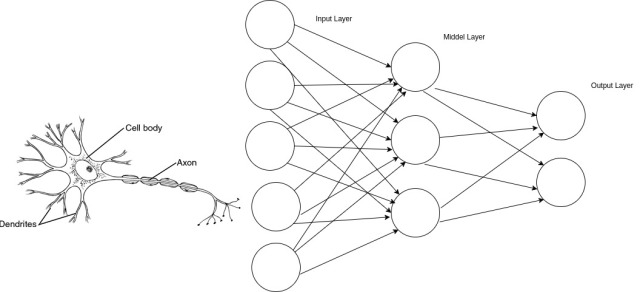
\includegraphics[scale=0.5]{neuralNet}
\end{frame}

\begin{frame}{What does machine learning means?}

  \begin{itemize}
\setlength\itemsep{1em}
\setbeamertemplate{itemize item}[triangle]
\setbeamercolor{itemize item}{fg=red}
  \item The concept of \texttt{training}
    \begin{itemize}
\setbeamertemplate{itemize subitem}[circle]
\setbeamercolor{itemize subitem}{fg=red}
    \item
      Minimize the loss
    \item    
      Loss functions
   \item
      Weights update
    \end{itemize}
  \item
    The importance of a large and well organized dataset
    \begin{itemize}
\setbeamertemplate{itemize subitem}[circle]
\setbeamercolor{itemize subitem}{fg=red}
    \item Common problems
    \item Cognitive bias
    \end{itemize}
  \end{itemize}
\end{frame}


\subsection{Tensorflow and OpenCv}

\begin{frame}{Tensorflow and OpenCv}
  \begin{itemize}
\setlength\itemsep{1em}
\setbeamertemplate{itemize item}[triangle]
\setbeamercolor{itemize item}{fg=red}
\item Tensorflow and computational graph concept
\end{itemize}
\begin{center}
    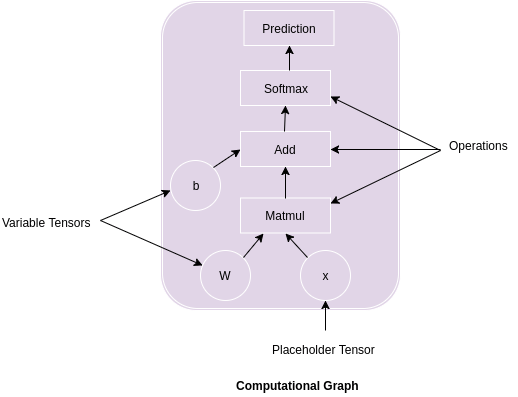
\includegraphics[scale=0.4]{comp}
\end{center}
%\begin{itemize}
%\item Low level and high level API
%\item OpenCv detection algorithm
%\end{itemize}
\end{frame}

\begin{frame}{Tensorflow and OpenCv}
\begin{itemize}
\setlength\itemsep{1em}
\setbeamertemplate{itemize item}[triangle]
\setbeamercolor{itemize item}{fg=red}
\item Low level and high level API
\begin{itemize}
\setbeamertemplate{itemize subitem}[circle]
\setbeamercolor{itemize subitem}{fg=red}
\item Tensorflow functions
\item Keras and tflearn
\end{itemize}
\item OpenCv "magic" detection algorithm
\begin{itemize}
\setbeamertemplate{itemize subitem}[circle]
\setbeamercolor{itemize subitem}{fg=red}
\item HaarCascadeClassifier
\item Dlib library for facial features detection
\end{itemize}
\end{itemize}
\end{frame}



\section{Image classification}

\subsection{Convolutional Neural Network}

\begin{frame}{Convolutional Neural Network}
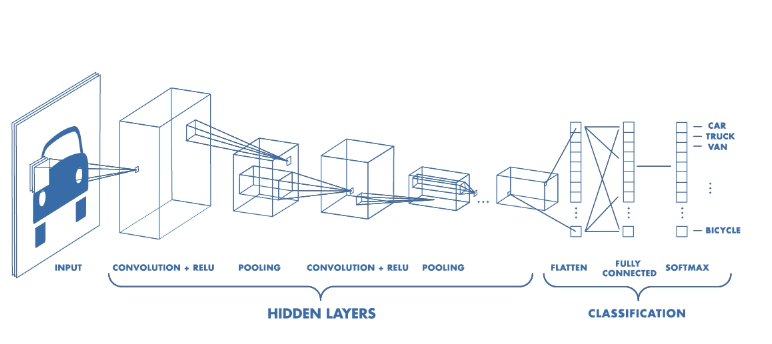
\includegraphics[scale=0.45]{CNN}
\end{frame}

\begin{frame}{Convolutional layers}
\begin{itemize}
\setlength\itemsep{1em}
\setbeamertemplate{itemize item}[triangle]
\setbeamercolor{itemize item}{fg=red}
\item Convolutional matrix (Kernel)
\end{itemize}
\begin{center}
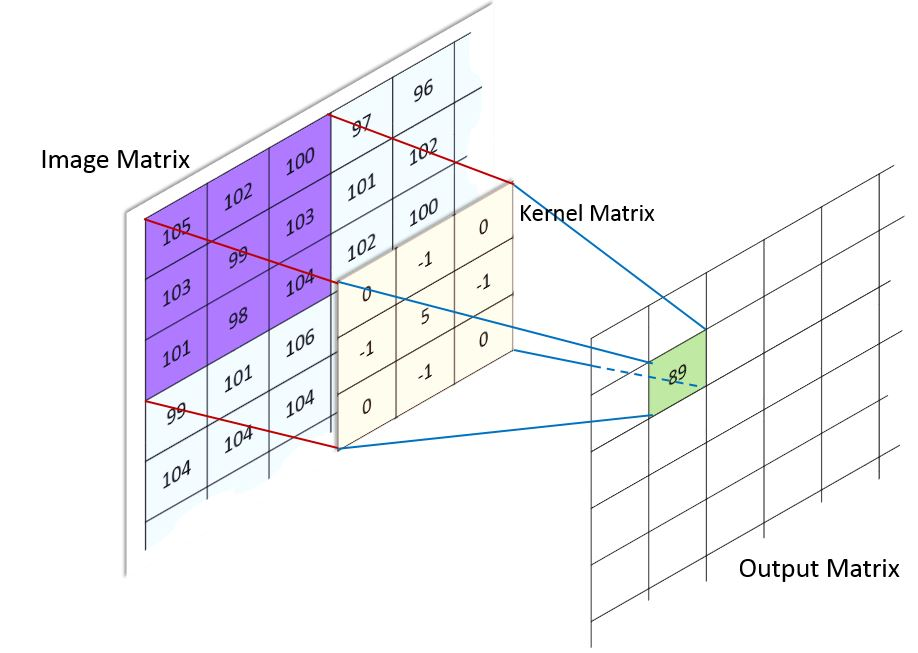
\includegraphics[scale=0.2]{kernel}
\end{center}
\begin{itemize}
\setlength\itemsep{1em}
\setbeamertemplate{itemize item}[triangle]
\setbeamercolor{itemize item}{fg=red}
\item 3x3, 5x5, or 7x7, why only odd numbers?
\item Edge detection
\begin{itemize}
\setbeamertemplate{itemize subitem}[circle]
\setbeamercolor{itemize subitem}{fg=red}
\item Similarity with human vision
\item From simple to complex forms
\end{itemize}
\end{itemize}
\end{frame}

\begin{frame}{Pooling layers}
\begin{itemize}
\setlength\itemsep{1em}
\setbeamertemplate{itemize item}[triangle]
\setbeamercolor{itemize item}{fg=red}
\item Reducing number of information: best way to avoiding \texttt{overfitting} and decreasing computation complexity
\end{itemize}
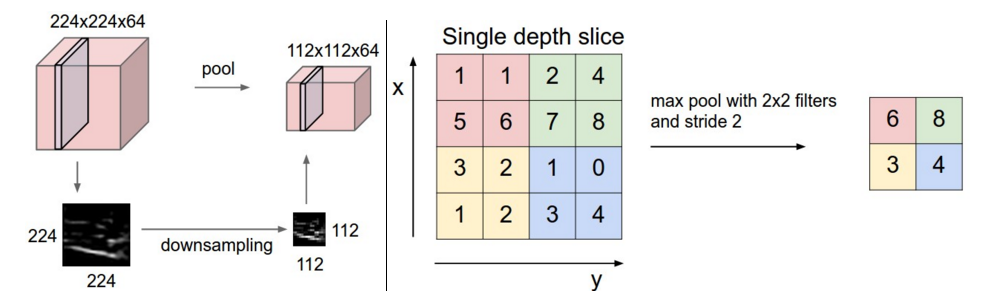
\includegraphics[scale=0.35]{pooling}
\end{frame}

\begin{frame}{Fully connected layers and dropout}
\begin{itemize}
\setlength\itemsep{1em}
\setbeamertemplate{itemize item}[triangle]
\setbeamercolor{itemize item}{fg=red}
\item Fully connected layers are the last layer of the CNN
\item Once the high-level features are recognized, they deal with classifications
\end{itemize}
\begin{center}
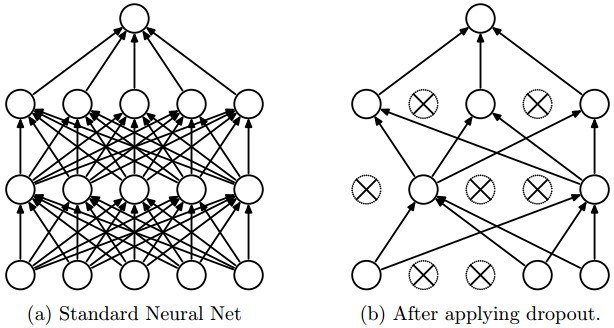
\includegraphics[scale=0.35]{dropout}
\end{center}
\end{frame}

\begin{frame}{Activation functions}
\begin{itemize}
\setlength\itemsep{1em}
\setbeamertemplate{itemize item}[triangle]
\setbeamercolor{itemize item}{fg=red}
\item ReLU
\end{itemize}
\begin{center}
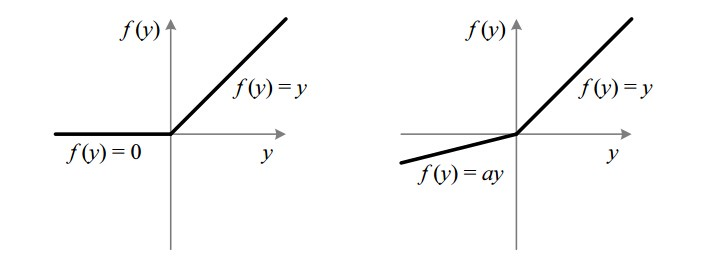
\includegraphics[scale=0.2]{ReLU}
\end{center}
\begin{itemize}
\setlength\itemsep{1em}
\setbeamertemplate{itemize item}[triangle]
\setbeamercolor{itemize item}{fg=red}
\item Softmax
\end{itemize}
\begin{center}
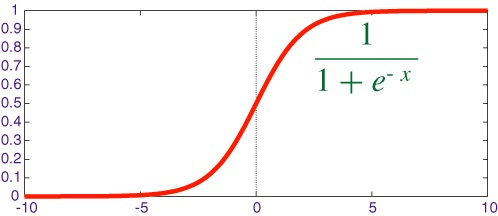
\includegraphics[scale=0.2]{softmax1}
\end{center}
\end{frame}


\subsection{Dataset}

\begin{frame}{Dataset}
\begin{itemize}
\setlength\itemsep{1em}
\setbeamertemplate{itemize item}[triangle]
\setbeamercolor{itemize item}{fg=red}
\item The perfect dataset should be:
\begin{itemize}
\setbeamertemplate{itemize subitem}[circle]
\setbeamercolor{itemize subitem}{fg=red}
\item made with hundreds of images
\item different images with different colors to help the network classify them better
\end{itemize}
\item The script use some OpenCv functions to get hundreds of photos in less than 30 seconds and, after that, crop them and saves them. This is made to avoid the recognitionof unwanted features as background color without the need of hundreds of images taken in different places
\end{itemize}
\end{frame}

\subsection{ImageNet}

\begin{frame}{ImageNet Challenge}
\begin{itemize}
\setlength\itemsep{1em}
\setbeamertemplate{itemize item}[triangle]
\setbeamercolor{itemize item}{fg=red}
\item The ImageNet project is a large visual database designed for use in visual object recognition software research. Over 14 million URLs of images have been hand-annotated by ImageNet to indicate what objects are pictured; in at least one million of the images, bounding boxes are also provided. ImageNet contains over 20 thousand categories; a typical category, such as "balloon" or "strawberry", contains several hundred images.
\item Since 2010, the annual ImageNet Large Scale Visual Recognition Challenge (ILSVRC) is a competition where research teams evaluate their algorithms on the given data set(ImageNet), and compete to achieve higher accuracy on several visual recognition tasks
\end{itemize}
\end{frame}

\subsection{Inception V3 by Google}

\begin{frame}{Inception network}
\begin{itemize}
\setlength\itemsep{1em}
\setbeamertemplate{itemize item}[triangle]
\setbeamercolor{itemize item}{fg=red}
\item Inception networks analize images with different kernel size (in the same conv layer)
\end{itemize}
\begin{center}
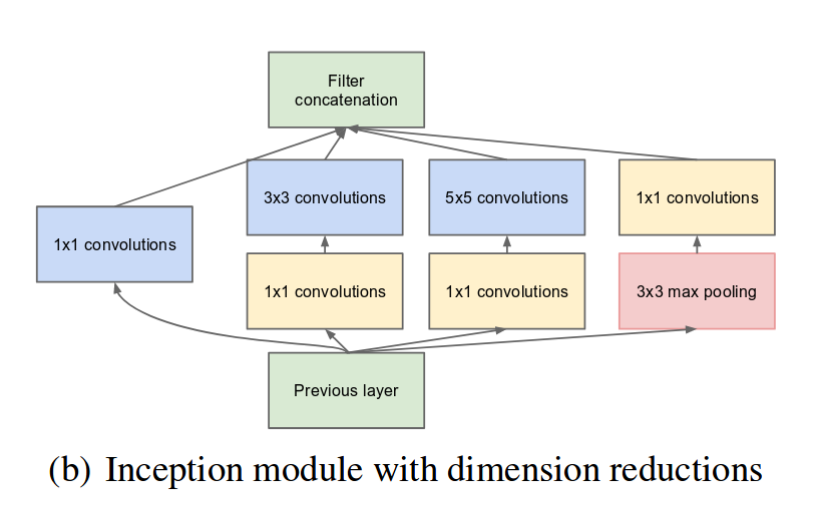
\includegraphics[scale=0.28]{inception}
\end{center}
\begin{itemize}
\setlength\itemsep{1em}
\setbeamertemplate{itemize item}[triangle]
\setbeamercolor{itemize item}{fg=red}
\item Here an example: \href{https://bit.ly/2vBgoO3}{GoogleNet}
\end{itemize}
\end{frame}

\subsection{Tensorflow and retraining}

\begin{frame}{Tensorflow and retraining}
\begin{itemize}
\setlength\itemsep{1em}
\setbeamertemplate{itemize item}[triangle]
\setbeamercolor{itemize item}{fg=red}
\item Concept of retraining
\item Tensorflow-hub: the key to create your own classifier with good result and without a tesla k80
\item Everything you need to know about retrain: \href{https://www.tensorflow.org/hub/tutorials/image_retraining}{tensorflow retraining}
\end{itemize}
\end{frame}

\section{Summary}

\subsection{Conclusion}
\begin{frame}{Conclusion}
\begin{itemize}
\setlength\itemsep{1em}
\setbeamertemplate{itemize item}[triangle]
\setbeamercolor{itemize item}{fg=red}
\item Create your own machine learning program using another pre-trained model can help you to build something useful without the need of a workstation or cloud computing
\item This project is only a small example of the potentiality of Tensorflow and the machine learning approach
\end{itemize}
\end{frame}

\subsection{Future implementation}

\begin{frame}{Future implementation}
\begin{itemize}
\setlength\itemsep{1em}
\setbeamertemplate{itemize item}[triangle]
\setbeamercolor{itemize item}{fg=red}
\item Let the users to choose beetwen more pre-trained models
\item Find the best way to recognize an unknown person (someone who does not have photos yet)
\end{itemize}
\end{frame}

\subsection{Best bugs}

\begin{frame}{Best bugs}
\begin{itemize}
\setlength\itemsep{1em}
\setbeamertemplate{itemize item}[triangle]
\setbeamercolor{itemize item}{fg=red}
\item OpenCv imshow freezing bug on unix like system
\item Tensorflow-hub requires a tensorflow version that could not work with lots of processors(precompiled with AVX activation)
\end{itemize}
\end{frame}

% All of the following is optional and typically not needed. 
\appendix
\section<presentation>*{\appendixname}
\subsection<presentation>*{Useful links}

\begin{frame}{Useful links}
\begin{itemize}
\setlength\itemsep{1em}
\setbeamertemplate{itemize item}[triangle]
\setbeamercolor{itemize item}{fg=red}
\item Project repository: \href{https://github.com/SimoneCaldarella/faceRecognition}{Link to repo}
\item Tensorflow: \href{https://www.tensorflow.org}{Link to Tensorflow page}
\item OpenCv: \href{https://opencv.org}{Link to OpenCv project}
\end{itemize}
\end{frame}

\end{document}


